%++++++++++++++++++++++++++++++++++++++++
% Don't modify this section unless you know what you're doing!
\documentclass[a4,11pt]{article}
\usepackage{pgfplots}
\usepackage{tabularx} % extra features for tabular environment
\usepackage{amsmath}  % improve math presentation
\usepackage{graphicx} % takes care of graphic including machinery
\usepackage[margin=1in,letterpaper]{geometry} % decreases margins
\usepackage{cite} % takes care of citations
\usepackage[final]{hyperref} % adds hyper links inside the generated pdf file
\usepackage{gensymb}
\usepackage{float}
\usepackage{appendix}
\hypersetup{
    colorlinks=true,       % false: boxed links; true: colored links
    linkcolor=blue,        % color of internal links
    citecolor=blue,        % color of links to bibliography
    filecolor=magenta,     % color of file links
    urlcolor=blue         
}
\makeatletter
\newcommand*{\rom}[1]{\expandafter\@slowromancap\romannumeral #1@}
\makeatother
%++++++++++++++++++++++++++++++++++++++++


\begin{document}
\twocolumn

\title{\Huge{Simple Displacement Sensor}\\
\Large{Catherine Beryl Basson and Piotr Chromi\'nski}\\
\large{13 December 2016}\\
\line(1,0){250}}
\date{}
\maketitle
\section{Introduction} \label{intro}

A displacement sensor is a device that can be used to measure position. There are numerous types of this sensor, which mainly fall into three categories: linear, multi-axis, and angular, which are used to measure displacement in one, multiple, or around an axis. This report will investigate use of a linear potentiometer as a angular displacement sensor.

\begin{figure}[h] 
  % read manual to see what [ht] means and for other possible options
  \centering
  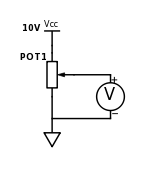
\includegraphics[width=0.5\columnwidth]{setup.png}
  % note that in above figure file name, "sr_setup",
  % the file extension is missing. LaTeX is smart enough to find
  % apropriate one (i.e. pdf, png, etc.)
  % You can add this extention yourself as it seen below
  % both notations are correct but above has more flexibility
  % \includegraphics[width=1.0\columnwidth]{sr_setup.pdf}
  \caption{
\label{fig:measurementsetup} % spaces are big no-no withing labels
    % things like fig: are optional in the label but it helps
    % to orient yourself when you have multiple figures,
    % equations and tables
    Measurement setup
  }
\end{figure}

A potentiometer can be used to  measure angular displacement in a
voltage divider configuration as shown in Figure \ref{fig:measurementsetup} where the potentiometer $POT1$ transduces rotation into voltage measured on the
washer terminal. It can be shown that voltage measured by the voltmeter is given by:
$$V_{M}=\frac{R_2R_L}{R_1R_L+R_1R_L+R_1R_2}\cdot V_{CC}$$
Where $V_{CC}$ is the voltage across the potentiometer, $R_1$ and $R_2$ are resistances from $V_{CC}$ to washer terminal and from washer terminal to ground, and $R_L$ is the input resistance of the voltmeter. Since typically $R_L\gg R_1+R_2$ $V_M$ can be approximated by:
$$V_{M}=\frac{R_2}{R_1+R_2}$$

As the potentiometer used in this experiment is linear, the model equation would yield an ideal straight line,
$$O(I)=KI+a$$
The ideal straight line for this equation can be determined by knowing the slope, K, and the y-intercept, a. It is hard to define the degrees that an ideal potentiometer would be able to turn, so it was assumed that the potentiometer would be able to turn from 0\degree\ to 360\degree. Additionally, it is assumed that ideally, when the potentiometer is set to 0\degree, the multimeter would read a value of 0V, and when it is set to it's maximum, it would read the full value of what was supplied to the circuit. This means that the y-intercept would be 0 in the ideal straight line.

The slope of the ideal straight line is given by the following:
$$K=\frac{O(I_{max})-O(I_{min})}{I_{max}-I_{min}}$$
In this experiment, the maximum voltage output will be 10V, and the minimum will be 0V. Along with the assumed lowest and highest angles of the potentiometer, this gives
$$K=\frac{10-0}{360-0}$$
$$K=0.02778$$
This makes the final ideal straight line equation
$$O_{ideal}(I)=0.02778(I)$$
\subsection{Hypothesis}
The main hypothesis for this experiment is that the potentiometer, when tested, would follow a linear path, and, provided the method of collecting data does not change, there would be consistency any collection error. Further, because of this, it is hypothesised that the test for the repeatability of this sensor will be successful, and that a clear bell curve will be seen from the data collected. It is assumed that there will be some error, both due to the way the data is collected, and the any static error from the manufacturing of the potentiometer.
\section{Experiments}
In this experiment, a potentiometer was attached to a printout of a circle with degrees, as seen in Figure \ref{fig:degcirc}. It was supplied with 10V from a power supply, and was adjusted so that what was seen as 180\degree\ (which is assumed to be the halfway point) would yield a reading of 5V on the multimeter.

\begin{figure}[h] 
	% read manual to see what [ht] means and for other possible options
	\centering
	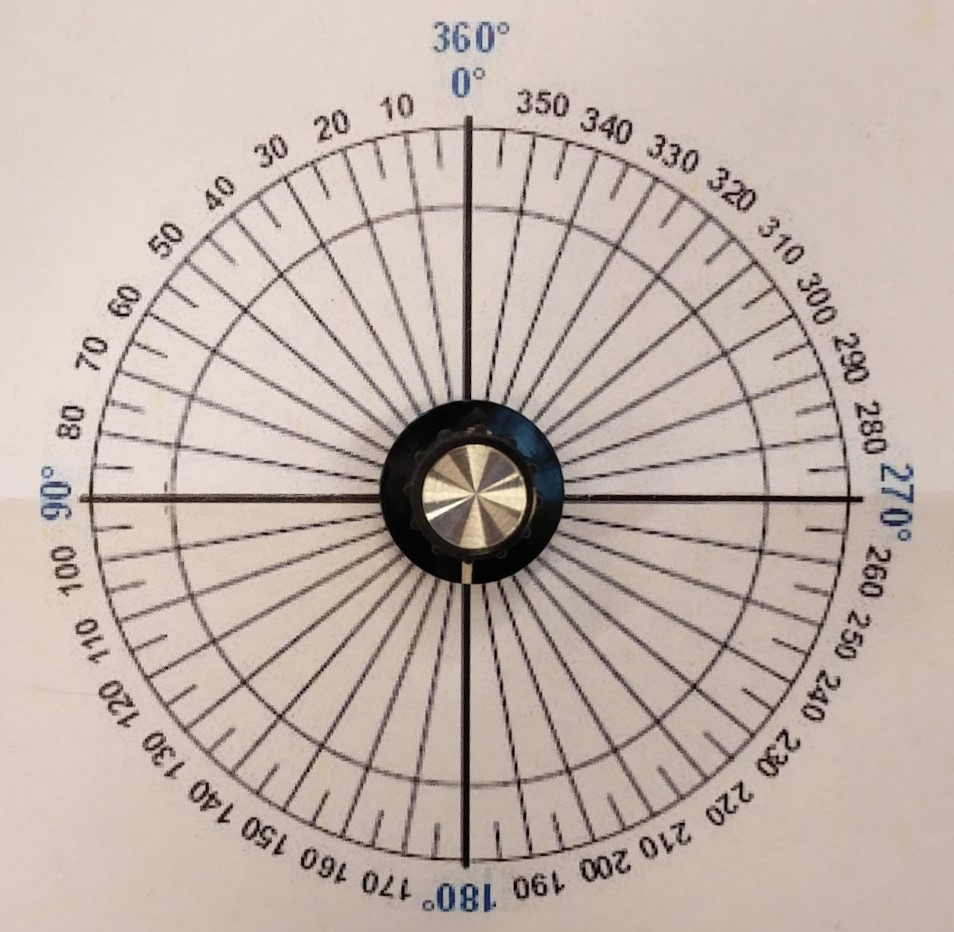
\includegraphics[width=0.75\columnwidth]{degcirc.png}
	% note that in above figure file name, "sr_setup",
	% the file extension is missing. LaTeX is smart enough to find
	% apropriate one (i.e. pdf, png, etc.)
	% You can add this extention yourself as it seen below
	% both notations are correct but above has more flexibility
	% \includegraphics[width=1.0\columnwidth]{sr_setup.pdf}
	\caption{
		\label{fig:degcirc} % spaces are big no-no withing labels
		% things like fig: are optional in the label but it helps
		% to orient yourself when you have multiple figures,
		% equations and tables
		Degree circle with potentiometer
	}
\end{figure}

First, the potentiometer was tested for linearity and hysteresis. This was done by starting the potentiometer as close to 0\degree\ as possible (in this case was 30\degree), and then increasing the degrees while taking note of the associated voltage. When the potentiometer maximum was reached, the same method was applied while going backwards in degrees. This was done three times, providing 6 groups of measurements. In the second and third run of this part of the experiment, fewer measurements were recorded, as it was decided to fix the increments/decrements to 30\degree. The information received from this part of the experiment will help to calculate the non-linearity of the potentiometer, which can be done by comparing the data to the ideal straight line determined in Section \ref{intro}. The hysteresis can be determined by analysing the data within a run, and comparing the half where the degree was increased with that from the half where the degree was decreased.

The next part of the experiment was done to test the potentiometer for repeatability. How this was done was by setting the potentiometer to 180\degree\ a total of 30 times (15 times from each extremity), and reading the value given by the potentiometer. Ideally, the potentiometer would read the same value every time, however as this is not the case in reality, a standard deviation can be calculated, which can help with determining a probability distribution function for the repeatability of the potentiometer.

The raw data from these experiments can will be presented in the Tables section of the Appendix.
\section{Results}
Here, the data from each part of this experiment are analysed and discussed. Important graphs, equations, and tables are shown directly in these subsections. Complete calculated data will be put into tables and graphs that can be seen in the Appendix.
\subsection{Hysteresis}
In order to calculate the hysteresis, the following equation is used:
$$H(I)=\lvert O_\downarrow-O_\uparrow\rvert$$
where $O_\uparrow$ is the output given at degree $I$ while going from min\degree\ to max\degree, and $O_\downarrow$ is the output given at degree $I$ while going the other way. This was done for every degree where the voltage was recorded from the multimeter for each run. So, for example, in the first run at $I=150\degree$, $O_\uparrow=3.922V$ and $O_\downarrow=3.96V$ which means that the hysteresis at this degree can calculated as such:
$$H(150)=\lvert 3.922-3.96\rvert$$
$$H(150)=0.038$$
After this is calculated for every value in a run, the maximum hysteresis, $\hat{H}$, is used to determine the maximum hysteresis as a percentage of full scale deflection:
$$\hat{H}\ as\ \%\ of\ f.s.d.=\frac{\hat{H}}{span}\cdot 100\%$$
where the span is $10V-0V=10V$. For example, in the first run $\hat{H}_1=0.659$, meaning
$$\hat{H}\ as\ \%\ of\ f.s.d.=\frac{0.659}{10}\cdot 100\%$$
$$\hat{H}\ as\ \%\ of\ f.s.d.=6.59\%$$
This was done for all three runs, and the full data is presented in Tables \ref{fig:firstsecond}, \ref{fig:thirdfourth}, and \ref{fig:fifthsixth} in the Appendix. The final maximum hysteresis' as a percentage of full scale deflection for the three runs are:
\begin{center}
	\begin{tabular}{c|c}
		Run Number & $\hat{H}\ as\ a\ \%\ of\ f.s.d$ \\
		\hline
		1 & 6.59\% \\
		2 & 9.88\% \\
		3 & 0.80\% \\
		\hline
	\end{tabular}
\end{center}
\subsection{Non-Linearity}
Next, the non-linearity of the data was calculated. This was done by looking at each set of data within the run separately, so the data collected when the degrees were increasing is independent from that where they are decreasing.
Non-linearity can be defined in terms of a function as:
$$N(I)=O_{actual}(I)-K(I)+a$$
where $O(I)$\ is the actual output at degree $I$\ and the expected output from the ideal straight line, $K(I)+a$\ is subtracted from it. The actual output equation is also written as
$$O_{actual}=K(I)+a$$
where, in this case, $K$ is the sensitivity of the potentiometer, and a is the theoretical y-intercept that would be reached if the potentiometer would be able to go to 0\degree, and if the output voltage was not restricted to 0V and 10V.

As, for the non-linearity, there are six sets of data, it was decided that in order to determine an average non-linearity equation, the sensitivity, $K$, and y-intercept, $a$, for each set of data would be determined, and then an average would be taken of $K$ and $a$ for all six sets, and put together into an average actual output equation.

The sensitivity is found by taking the slope of the data, so
$$K=\frac{dO}{dI}$$
This was not computed by hand, but rather by Excel. The y-intercept is found by
$$a=O(I_{min})-KI_{min}$$
i.e. multiplying the sensitivity of a given set of data by the actual minimum input degree, $30\degree$\ and subtracting it from the output voltage at this input, $0V$. For example, in the first run, the sensitivity is calculated to be $K=0.03884$, so the y-intercept is
$$a=0-0.03884\times30$$
$$a=-1.1652$$
The following table shows the calculated sensitivities and y-intercepts for each set of data:
\begin{center}
	\begin{tabular}{c|c|c}
		Set Number & Sensitivity, $K$ & y-intercept, $a$ \\
		\hline
		1 & 0.03884 & -1.1652 \\
		2 & 0.03880 & -1.1640 \\
		3 & 0.03793 & -1.1377 \\
		4 & 0.03852 & -1.1555 \\
		5 & 0.03772 & -1.1315 \\
		6 & 0.03776 & -1.1329 \\
		\hline
	\end{tabular}
\end{center}

Next, the average sensitivity
$$\bar{K}= \frac{1}{N}\sum_{i}^{n}{K_i}$$
and the average y-intercept
$$\bar{a}= \frac{1}{N}\sum_{i}^{n}{a_i}$$
were calculated. This yields $\bar{K}=0.038$ as the sensitivity and $\bar{a}=-1.14$ and the y-axis, making the average output function:
$$O_{actual}=0.038(I)-1.14$$
In order to compare the average actual output equation to that of the ideal straight line equation to determine non-linearity, values from 30\degree\ to 270\degree, with increments of 30\degree, were substituted into $O_{actual}$. This was because, outside of this domain, the output voltage was either below 0V or above 10V, and therefore not valid or possible with the setup from this experiment. The results from this can be seen in Table \ref{idealandact}. In Figure \ref{fig:actual}, a graph is shown to display how the average actual output voltage differs from the ideal straight line. Here, the percentage error bands are also displayed, and this will be discussed in the Error Discussion section.	

\begin{figure}[h]
	\centering
	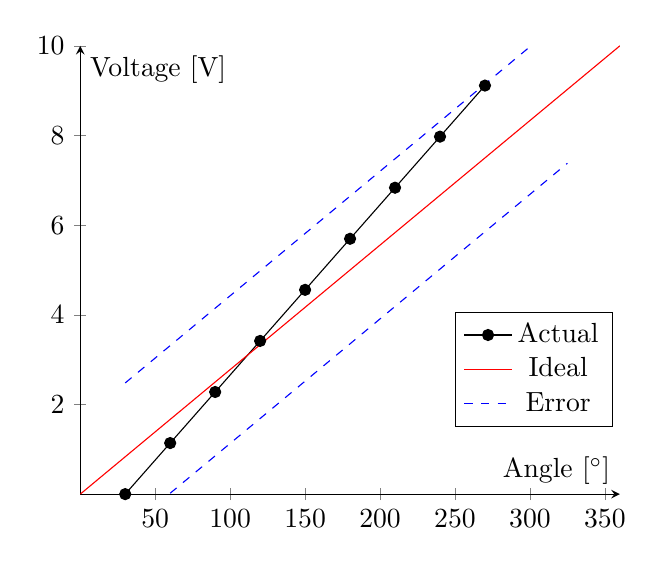
\begin{tikzpicture}
	\begin{axis}[
	axis lines=middle,
	legend style={at={(axis cs:250,1.5)},
		anchor=south west},
	xlabel=Angle \lbrack \degree \rbrack, ylabel=Voltage \lbrack V\rbrack]
	\addplot[smooth,
	color=black,
	mark=*,
	error bars/.cd,y dir=both,
	y explicit
	] coordinates {
		(30, 0)
		(60, 1.139138804)
		(90, 2.278277607)
		(120, 3.417416411)
		(150, 4.556555215)
		(180, 5.695694018)
		(210, 6.834832822)
		(240, 7.973971626)
		(270, 9.113110429)
	};
	\addlegendentry{Actual}
	\addplot[draw=red][domain=0:360]{0.027778*x};
	\addplot[draw=blue, dashed][domain=30:300]{0.027778*x+1.64667};
	\addplot[draw=blue, dashed][domain=60:325]{0.027778*x-1.64667};
	\addlegendentry{Ideal}
	\addlegendentry{Error}
	\end{axis}
	\end{tikzpicture}
	\label{fig:actual}
	Figure 3.2: Average Actual Output Compared to Ideal Straight Line
\end{figure}

The non-linearity is then calculated for each input data point. For example, at $I=150\degree$, the non-linearity is
$$N(150)=4.5566-4.1667$$
$$N(150)=0.3899$$
A full table of this data can be seen in Table \ref{idealandact} in the Appendix. From the calculations, the maximum non-linearity, $\hat{N}$, is seen to be 2.530527, and from this, the maximum non-linearity as a percentage of full scale deflection can be calculated as follows:
$$\hat{N}\ as\ \%\ of\ f.s.d=\frac{\hat{N}}{O_{max}-O_{min}}\cdot 100\%$$
where $O_{max}$ and $O_{min}$ are taken from the actual data output. So,
$$\hat{N}\ as\ \%\ of\ f.s.d=\frac{2.5305}{12.5305+1.1391}\cdot 100\%$$
$$\hat{N}\ as\ \%\ of\ f.s.d=18.51\%$$
\subsection{Repeatability}
In order to analyse the repeatability of this potentiometer, the data collected in the second part of this experiment was separated into intervals between 4.9V and 5.2V, increasing by 0.05V each time, in order to determine the frequency of an occurrence in each interval. In theory, the majority of occurrences would happen closest to the centre, forming a bell curve, known as a probability distribution function. The estimated voltage for the centre value is 5V, as this is what was used to calibrate the potentiometer at the beginning of this experiment, and the potentiometer is being turned to 180\degree, the estimated centre, each time. Figure \ref{fig:histogram}.1 on the following page is a histogram demonstrating the distribution of frequency from this repeatability.

\begin{figure}[h]
	\centering
	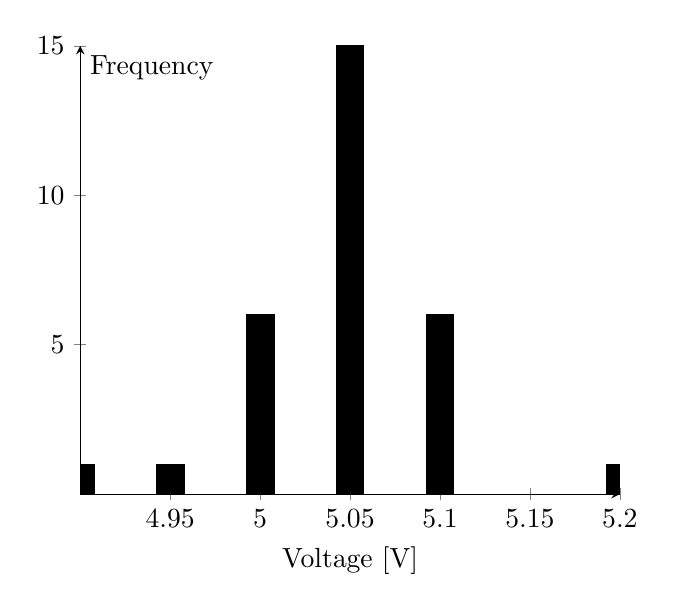
\begin{tikzpicture}
	\begin{axis}[axis lines=middle,
	xlabel near ticks,
	xlabel=Voltage \lbrack V\rbrack, ylabel=Frequency]
	\addplot[ybar,fill=black] coordinates {
		(4.9, 1)
		(4.95, 1)
		(5, 6)
		(5.05, 15)
		(5.1, 6)
		(5.15, 0)
		(5.2, 1)
	};
	\end{axis}
	\end{tikzpicture}
	\label{fig:histogram}
	Figure 3.3.1: Histogram
\end{figure}

In order to determine a probability distribution function, the probability density must first be calculated. This is first done by determining the probability that a given data set will fall into a given interval, i.e.
$$P_x=\frac{n}{30}$$
where $n$ is the number of occurrences in the given frequency, and $30$ is the total number of data points collected. So, for example, in the 5-5.05V interval, there were six occurrences, meaning that the probability of any given data point falling into this interval is
$$P_x=\frac{6}{30}$$
$$P_x=0.2$$
Next, the probability density, $P_n$ is calculated
$$P_n=\frac{P_x}{0.05}$$
where $P_x$ is the aforementioned probability, and $0.05$ is the interval width. So, again for the 5-5.05V interval, the probability density is
$$P_n=\frac{0.2}{0.05}$$
$$P_n=4$$
Table \ref{histprob} in the Appendix shows the intervals, frequency, probability, and probability density.
In order to plot probability density, which is on the y-axis of a graph, the standard deviation of the data is needed. In order to do this, it is first required to find the average of the data.
$$\bar{x}=\frac{1}{30}\sum_{i}^{n}{x_i}$$
$$\bar{x}=5.02567$$
and from this, the standard deviation
$$\sigma=\sum_{i}^n{\sqrt{\frac{(x_i-\bar x)^2}{n}}}$$
$$\sigma=0.04673$$
So, from this, a probability distribution function can be plotted, where each step away from the highest probability density is an additional standard deviation on the x-axis. In Figure \ref{fig:probdens}.2, the probability distribution function is shown.
\begin{figure}[H]
	\centering
	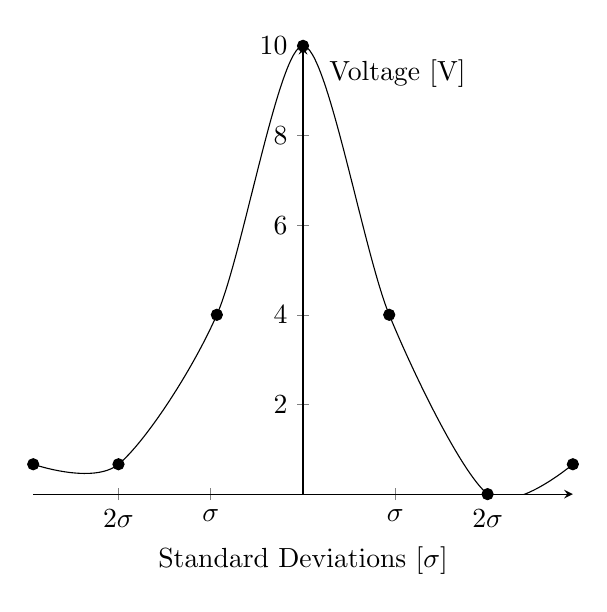
\begin{tikzpicture}
	\begin{axis}[
	axis lines=middle,
	ylabel style={at={(ticklabel cs:0.99,-25)}},
	xlabel near ticks,
	xlabel=Standard Deviations \lbrack $\sigma$\rbrack, ylabel=Voltage \lbrack V\rbrack,
	xticklabels={,$2\sigma$,$\sigma$,,$\sigma$,$2\sigma$}]
	\addplot[smooth,color=black,mark=*] coordinates {
		(-0.1462, 0.6667)
		(-0.100, 0.6667)
		(-0.0467, 4)
		(0, 10)
		(0.0467, 4)
		(0.100, 0)
		(0.1462, 0.6667)
	};
	\end{axis}
	\end{tikzpicture}
	\label{fig:probdens}
	Figure: 3.3.2: Probability Density Function
\end{figure}

\section{Error Discussion}
Here, the results and error for each part of the experiments. Before they are discussed individually, there are some overall errors from the experiment that can be discussed. For example, when collecting the data, depending on how the potentiometer and degree circle are looked at, there may be some parallax error, which results in the possibility of the degree not being read accurately, or set precisely. Furthermore, there is some tolerance on the multimeter that may result in some error when reading the output of the setup. Additionally, while the potentiometer was stationary, the voltage read on the multimeter would still fluctuate by approximately $\pm0.01V$, meaning that the voltage noted for a given degree may vary. While this fluctuation is small, as it is applied to every measurement, the error increases. Finally, when using the potentiometer and degree circle, the degree circle may have become loosened or out of place, adding some offset for a read value of a given degree.
\subsection{Hysteresis}
It is noticed that, for the three runs, there was no similarities in the maximum hysteresis as a percentage of f.s.d.. Additionally, the only noticeable hysteresis happens in the first and second run at $I=120\degree$. At the majority of the other input degrees, the difference in output voltage when going forward and that when going back is negligible, as they are not noticeable on the graphs in Figure \ref{fig:firstsecond} and \ref{fig:thirdfourth} from the Appendix. It is suspected that this may be due to some manufacturing factors, for example the stiffness of the potentiometer, which may have affected how the knob was turned relative to the circle with degrees nearing one extreme.
\subsection{Non-Linearity}
Despite the data not following the slope of the ideal straight line, the potentiometer remains reasonably linear throughout the experiments. Obviously, when comparing the average actual output plot to the ideal straight line plot, the non-linearity will be at its highest the farther away from the intersecting point, and this is the nature of non-parallel lines. However, it is noted that, as this average actual output was calculated as a straight line equation, the non-linearity is taken relative to the ideal straight line, and not in the non-linearity of the equation itself. Another possible way to determine the non-linearity would have been to take an average of the output data collected at each degree, and then found the sensitivity and y-intercept of these averages. From this, another total non-linearity can be determined, and compared to the ideal straight line.	

When determining the error bands, it was decided that they would be given the value of $\pm$\ the maximum non-linearity from the entire set of data. This was found to be at every output point collected at $I=330\degree$. So, the error bands are $\pm1.6466$ from the ideal straight line. The error bars also only are visible between degrees that would allow for the output value to remain between 0V and 10V, as outside this range would not be possible. When the output equation is also limited to the input degrees that would output between this range (30\degree\ and 270\degree), it is seen that this line falls between the error bars.

One noticeable point of error during this part of the experiment is that, while it is expected that the voltage value would be constantly changing with the change in degree, however this was not the case. At both extremities of the potentiometer, there was some delay before the multimeter would read a value other than 0V at the lower extremity, and 10V at the higher one. Had this been included in the calculations, this would have affected the line of best fit for the results.
\subsection{Repeatability}
The behaviour of the repeatability acts as expected, forming a bell curve in the probability density function. The reason for any outliers, and for why the data points are not closer to the ideal centre, can be linked to parallax error and small changes in the configuration of the potentiometer and degree circle. However, overall, any error in this part of the experiment is negligible, and the potentiometer has a decent repeatability.
\section{Conclusion}
 This experiment had two main hypotheses. First, while recording data for the hysteresis and non-linearity part of the experiment, these results would turn out to follow a linear trend within each set of data. Second, while recording data for the repeatability of the potentiometer, the data would form a bell curve on a probability density function. Overall, both of these expectations were met through the methods used to analyse the data, and the experiments have therefore confirmed the hypotheses of this lab assignment.
 
 In the first part of the experiment, both when the sets of data are looked at separately and combined, they showed similar linear trends on a graph. Additionally, namely in Run \rom{1} and Run \rom{2}, they appeared to have similar deviations occurring at the same inputs, for example when analysing hysteresis, pushing the conclusion that some error in the function of this potentiometer may be manufacturer based, or due to a faulty component. If these points are considered to be outliers and thereby negated, then the trend can be seen as fully linear, where any small non-linearity on each individual data set can be attributed to static error or some error in data collection. The non-linearity in relation to the ideal straight line can be related to the nature of the potentiometer, where, for one, the potentiometer does not turn 360\degree, and 
 
 In the second part of the experiment, both the histogram and the probability density function behaved as expected. Any outliers further away from the centre value can be accredited to faults data collection such as parallax error or tolerance in the multimeter.

For future renditions of this lab experiment, as well as in applications of this potentiometer, it is recommended to take more limit the operational range of this potentiometer to be further away from its extremities, for example between 25\degree and 250\degree relative to the start and end points of the potentiometer. Within a range similar to this, it is expected that a change in the angle would result in a noticeable change in voltage, rather than the constant voltage noticed at any changes by the extremities. This will reduce some error caused by gathering data before and after the potentiometer's effective range, for example by making a line of best fit more similar to the ideal straight line.
\onecolumn
\begin{thebibliography}{99}
	
	\bibitem{SAA}
	J.P.\ Bentley, \textit{Principles of Measurement Systems, 4th Edition},
	(Pearson Education Limited, England, 2005).
	
	\bibitem{Wiki} \emph{Potentiometer},   available at
	\texttt{https://en.wikipedia.org/wiki/Potentiometer}.
	
\end{thebibliography}
\appendix
\section{Tables}
\begin{table}[H]
	\centering
	\caption{Hysteresis Data \rom{1}}
	\label{hyst1}
	\begin{tabular}{l|l|l||l}
		Angle $[^{\circ}]$  &  $30^{\circ}\rightarrow325^{\circ}$  \
		&  $325^{\circ}\rightarrow30^{\circ}$  &  $H(I) [V]$  \\
		\hline
		30  &  0  &  0  &  0  \\
		35  &  0  &  0  &  0  \\
		40  &  0  &  0  &  0  \\
		45  &  0.005  &  0.006  &  0.001  \\
		50  &  0.01  &  0.011  &  0.001  \\
		60  &  0.03  &  0.027  &  0.003  \\
		70  &  0.473  &  0.443  &  0.03  \\
		80  &  0.877  &  0.988  &  0.111  \\
		90  &  1.377  &  1.498  &  0.121  \\
		120  &  2.842  &  2.183  &  0.659  \\
		150  &  3.922  &  3.96  &  0.038  \\
		180  &  4.98  &  4.97  &  0.01  \\
		210  &  6.21  &  6.18  &  0.03  \\
		240  &  7.53  &  7.53  &  0  \\
		270  &  9.04  &  8.87  &  0.17  \\
		280  &  9.38  &  9.41  &  0.03  \\
		290  &  9.92  &  9.83  &  0.09  \\
		295  &  9.98  &  9.97  &  0.01  \\
		300  &  9.98  &  9.98  &  0  \\
		305  &  9.99  &  9.99  &  0  \\
		310  &  10  &  10  &  0  \\
		325  &  10  &  10  &  0  \\
	\end{tabular}
\end{table}

\begin{table}[H]
	\centering
	\caption{Hysteresis Data \rom{2}}
	\label{hyst2}
	\begin{tabular}{l|l|l||l}
		Angle $[^{\circ}]$  &  $30^{\circ}\rightarrow325^{\circ}$  \
		&  $325^{\circ}\rightarrow30^{\circ}$  &  $H(I) [V]$  \\
		\hline
		30  &  0  &  0  &  0  \\
		60  &  0.025  &  0.065  &  0.04  \\
		90  &  1.414   &  1.383  &  0.031  \\
		120  &  2.806  &  1.818  &  0.988  \\
		150  &  4.02  &  3.92  &  0.1  \\
		180  &  5.03  &  5.01  &  0.02  \\
		210  &  6.21  &  6.13  &  0.08  \\
		240  &  7.51  &  7.45  &  0.06  \\
		270  &  8.98  &  9.02  &  0.04  \\
		300  &  9.98  &  9.98  &  0  \\
		325  &  10  &  10  &  0  \\
	\end{tabular}
\end{table}

\begin{table}[H]
	\centering
	\caption{Hysteresis Data \rom{3}}
	\label{hyst3}
	\begin{tabular}{l|l|l||l}
		Angle $[^{\circ}]$  &  $30^{\circ}\rightarrow325^{\circ}$  \
		&  $325^{\circ}\rightarrow30^{\circ}$  &  $H(I) [V]$  \\
		\hline
		30  &  0  &  0  &  0  \\
		60  &  0.093  &  0.114  &  0.021  \\
		90  &  1.446  &  1.404  &  0.042  \\
		120  &  2.831  &  2.874  &  0.043  \\
		150  &  3.959  &  3.95  &  0.009  \\
		180  &  5.04  &  5.01  &  0.03  \\
		210  &  6.27  &  6.29  &  0.02  \\
		240  &  7.42  &  7.5  &  0.08  \\
		270  &  8.91  &  8.91  &  0  \\
		300  &  9.98  &  9.98  &  0  \\
		325  &  10  &  10  &  0  \\
	\end{tabular}
\end{table}

\begin{table}[H]
	\centering
	\caption{Ideal Straight Line and Actual}
	\label{idealandact}
	\begin{tabular}{l|l|l|l}
		Angle  &  $V_{Ideal}$  &  $V_{Average Actual}$  &  $N(I)$  \\  \hline
		0  &  0  &  -1.1391  &  1.1391  \\
		30  &  0.8333  &  0  &  0.8333  \\
		60  &  1.6667  &  1.1391  &  0.5275  \\
		90  &  2.5  &  2.2783  &  0.2217  \\
		120  &  3.3333  &  3.4174  &  0.08408  \\
		150  &  4.1667  &  4.5566  &  0.3899  \\
		180  &  5  &  5.6957  &  0.6957  \\
		210  &  5.8333  &  6.8348  &  1.001499  \\
		240  &  6.6667  &  7.9740  &  1.3073  \\
		270  &  7.5  &  9.1131  &  1.6131  \\
		300  &  8.3333  &  10.2522  &  1.9189  \\
		330  &  9.1667  &  11.3914  &  2.2247  \\
		360  &  10  &  12.5305  &  2.5305  \\
	\end{tabular}
\end{table}

\begin{table}[H]
	\centering
	\caption{Repeatability Data [V]}
	\label{repeat}
	\begin{tabular}{l|l|l}
		4.99  &  5.07  &  5.01  \\
		5.01  &  5.1  &  4.98  \\
		5.04  &  5.04  &  4.97  \\
		5.04  &  4.93  &  4.98  \\
		5.02  &  5.04  &  5.02  \\
		5.11  &  5  &  5.06  \\
		5.04  &  4.9  &  5.05  \\
		5.06  &  5.09  &  5.04  \\
		5.04  &  5.04  &  5.03  \\
		5.01  &  5.08  &  4.98  \\
	\end{tabular}
\end{table}

\begin{table}[H]
	\centering
	\caption{Histogram/Probability Density Data}
	\label{histprob}
	\begin{tabular}{l|l||l|l}
		Interval  &  Freq.  &  $P_x=\frac{f}{30}$  &  $P_n=\frac{P}{0.05}$\\  \hline
		4.9   &  1  &  0.03333  &  0.6667 \\
		4.95  &  1  &  0.03333  &  0.6667 \\
		5  &  6  &  0.2  &  4 \\
		5.05  &  15  &  0.5  &  10 \\
		5.1  &  6   &  0.2  &  4 \\
		5.15  &  0   &  0  &  0 \\
		5.2  &  1  &  0.03333  &  0.6667 \\
	\end{tabular}
\end{table}

\section{Graphs}
\begin{figure}[H]
	\centering
	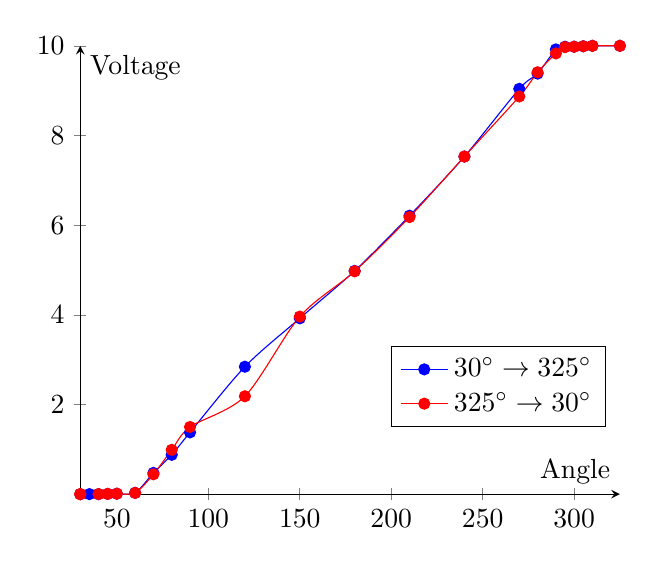
\begin{tikzpicture}
	\begin{axis}[axis lines=middle,
	legend style={at={(axis cs:200,1.5)},
		anchor=south west},
	xlabel=Angle, ylabel=Voltage]
	\addplot[smooth,color=blue,mark=*] coordinates {
		(30, 0)
		(35, 0)
		(40, 0)
		(45, 0.005)
		(50, 0.01)
		(60, 0.03)
		(70, 0.473)
		(80, 0.877)
		(90, 1.377)
		(120, 2.842)
		(150, 3.922)
		(180, 4.98)
		(210, 6.21)
		(240, 7.53)
		(270, 9.04)
		(280, 9.38)
		(290, 9.92)
		(295, 9.98)
		(300, 9.98)
		(305, 9.99)
		(310, 10)
		(325, 10)
	};
	\addlegendentry{$30^{\circ} \rightarrow 325^{\circ}$}
	\addplot[smooth,color=red,mark=*] coordinates {
		(30, 0)
		(30, 0)
		(40, 0)
		(45, 0.006)
		(50, 0.011)
		(60, 0.027)
		(70, 0.443)
		(80, 0.988)
		(90, 1.498)
		(120, 2.183)
		(150, 3.96)
		(180, 4.97)
		(210, 6.18)
		(240, 7.53)
		(270, 8.87)
		(280, 9.41)
		(290, 9.83)
		(295, 9.97)
		(300, 9.98)
		(305, 9.99)
		(310, 10)
		(325, 10)
	};
	\addlegendentry{$325^{\circ} \rightarrow 30^{\circ}$}
	\end{axis}
	\end{tikzpicture}
	\caption{Run \rom{1}}
	\label{fig:firstsecond}
\end{figure}

\begin{figure}[H]
	\centering
	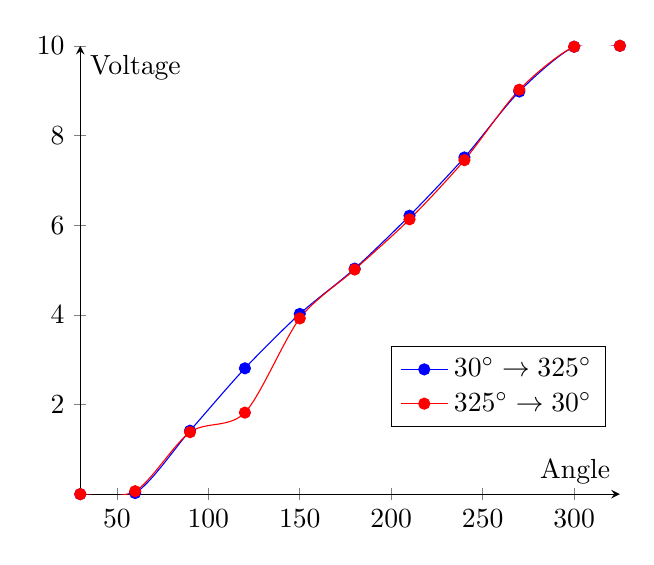
\begin{tikzpicture}
	\begin{axis}[
	axis lines=middle,
	legend style={at={(axis cs:200,1.5)},
		anchor=south west},
	xlabel=Angle, ylabel=Voltage]
	\addplot[smooth,color=blue,mark=*] coordinates {
		(30, 0)
		(60, 0.025)
		(90, 1.414)
		(120, 2.806)
		(150, 4.02)
		(180, 5.03)
		(210, 6.21)
		(240, 7.51)
		(270, 8.98)
		(300, 9.98)
		(325, 10)
	};
	\addlegendentry{$30^{\circ} \rightarrow 325^{\circ}$}
	\addplot[smooth,color=red,mark=*] coordinates {
		(30, 0)
		(60, 0.065)
		(90, 1.383)
		(120, 1.818)
		(150, 3.92)
		(180, 5.01)
		(210, 6.13)
		(240, 7.45)
		(270, 9.02)
		(300, 9.98)
		(325, 10)
	};
	\addlegendentry{$325^{\circ} \rightarrow 30^{\circ}$}
	\end{axis}
	\end{tikzpicture}
	\caption{Run \rom{2}}
	\label{fig:thirdfourth}
\end{figure}

\begin{figure}[H]
	\centering
	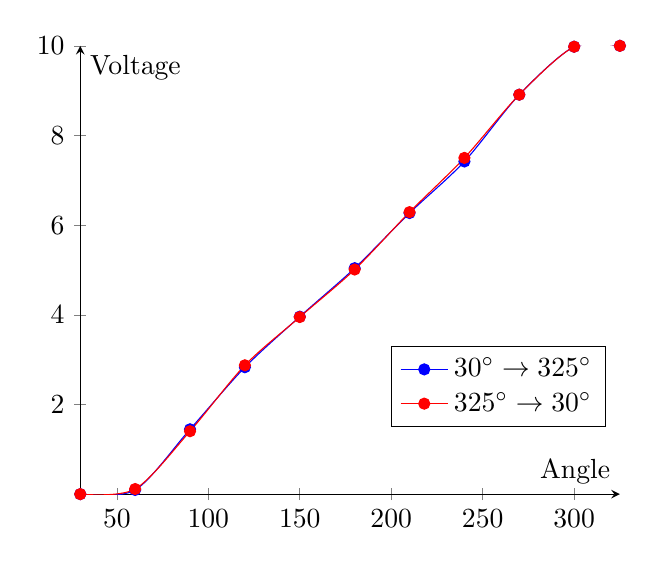
\begin{tikzpicture}
	\begin{axis}[
	axis lines=middle,
	legend style={at={(axis cs:200,1.5)},
		anchor=south west},
	xlabel=Angle, ylabel=Voltage]
	\addplot[smooth,color=blue,mark=*] coordinates {
		(30, 0)
		(60, 0.093)
		(90, 1.446)
		(120, 2.831)
		(150, 3.959)
		(180, 5.04)
		(210, 6.27)
		(240, 7.42)
		(270, 8.91)
		(300, 9.98)
		(325, 10)
	};
	\addlegendentry{$30^{\circ} \rightarrow 325^{\circ}$}
	\addplot[smooth,color=red,mark=*] coordinates {
		(30, 0)
		(60, 0.114)
		(90, 1.404)
		(120, 2.874)
		(150, 3.95)
		(180, 5.01)
		(210, 6.29)
		(240, 7.5)
		(270, 8.91)
		(300, 9.98)
		(325, 10)
	};
	\addlegendentry{$325^{\circ} \rightarrow 30^{\circ}$}
	\end{axis}
	\end{tikzpicture}
	\caption{Run \rom{3}}
	\label{fig:fifthsixth}
\end{figure}

\end{document}
